\documentclass[aspectratio=169,11pt]{beamer}
\usepackage[spanish]{babel}
\usepackage[utf8]{inputenc}
\usepackage[T1]{fontenc}
\usepackage{lmodern}
\usepackage{tikz}
\usetikzlibrary{arrows.meta,positioning}

\usetheme{default}
\setbeamertemplate{navigation symbols}{}
\setbeamertemplate{footline}[frame number]
\definecolor{acento}{RGB}{0,92,151}
\definecolor{gris}{RGB}{120,120,120}
\setbeamercolor{frametitle}{fg=acento}
\setbeamercolor{title}{fg=acento}
\setbeamercolor{itemize item}{fg=acento}
\setbeamerfont{frametitle}{series=\bfseries}

\graphicspath{{../../reports/figures/}}

% Barras simples en TikZ puro: #1 título, #2 máximo del eje, #3-#5 valores (azar, sin entrenar, entrenado)
\newcommand{\barras}[5]{%
\begin{tikzpicture}[x=1.7cm,y=1cm]
  \def\alto{3.2}
  \foreach \v/\lab [count=\i] in {#3/Azar,#4/Sin entrenar,#5/Entrenado}{
    \pgfmathsetmacro{\hh}{\v/#2*\alto}
    \fill[acento!70] (\i-0.3,0) rectangle (\i+0.3,\hh);
    \node[above,font=\scriptsize] at (\i,\hh) {\v};
    \node[below,font=\footnotesize] at (\i,0) {\lab};
  }
  \draw[gris!60] (0.4,0) -- (3.6,0);
  \node[font=\small\bfseries] at (2,\alto+0.7) {#1};
\end{tikzpicture}}

\title{Localización del LCA en resonancias de rodilla}
\subtitle{Avance de resultados: ¿dónde mira el modelo?}
\author{Christopher Zúñiga, C28730}
\institute{CI-0148 Aprendizaje Automático --- Universidad de Costa Rica}
\date{20 de noviembre de 2026}

\begin{document}

\begin{frame}
  \titlepage
\end{frame}

% -------------------------------------------------------------------------
\begin{frame}{El problema}
  \begin{itemize}
    \item \textbf{Objetivo:} encontrar automáticamente el ligamento cruzado anterior (LCA)
          dentro de una resonancia de rodilla, es decir, predecir la caja 3D que lo contiene.
    \item Es el primer paso antes de evaluar si el ligamento está sano, parcialmente lesionado o roto.
    \item \textbf{Datos:} KneeMRI, 917 resonancias sagitales con caja anotada a mano
          (75\,\% sanos, 19\,\% parciales, 6\,\% rotos).
    \item El LCA aparece solo en 2--6 de los 21--45 cortes de cada volumen.
  \end{itemize}
  \vspace{0.3em}
  \centering
  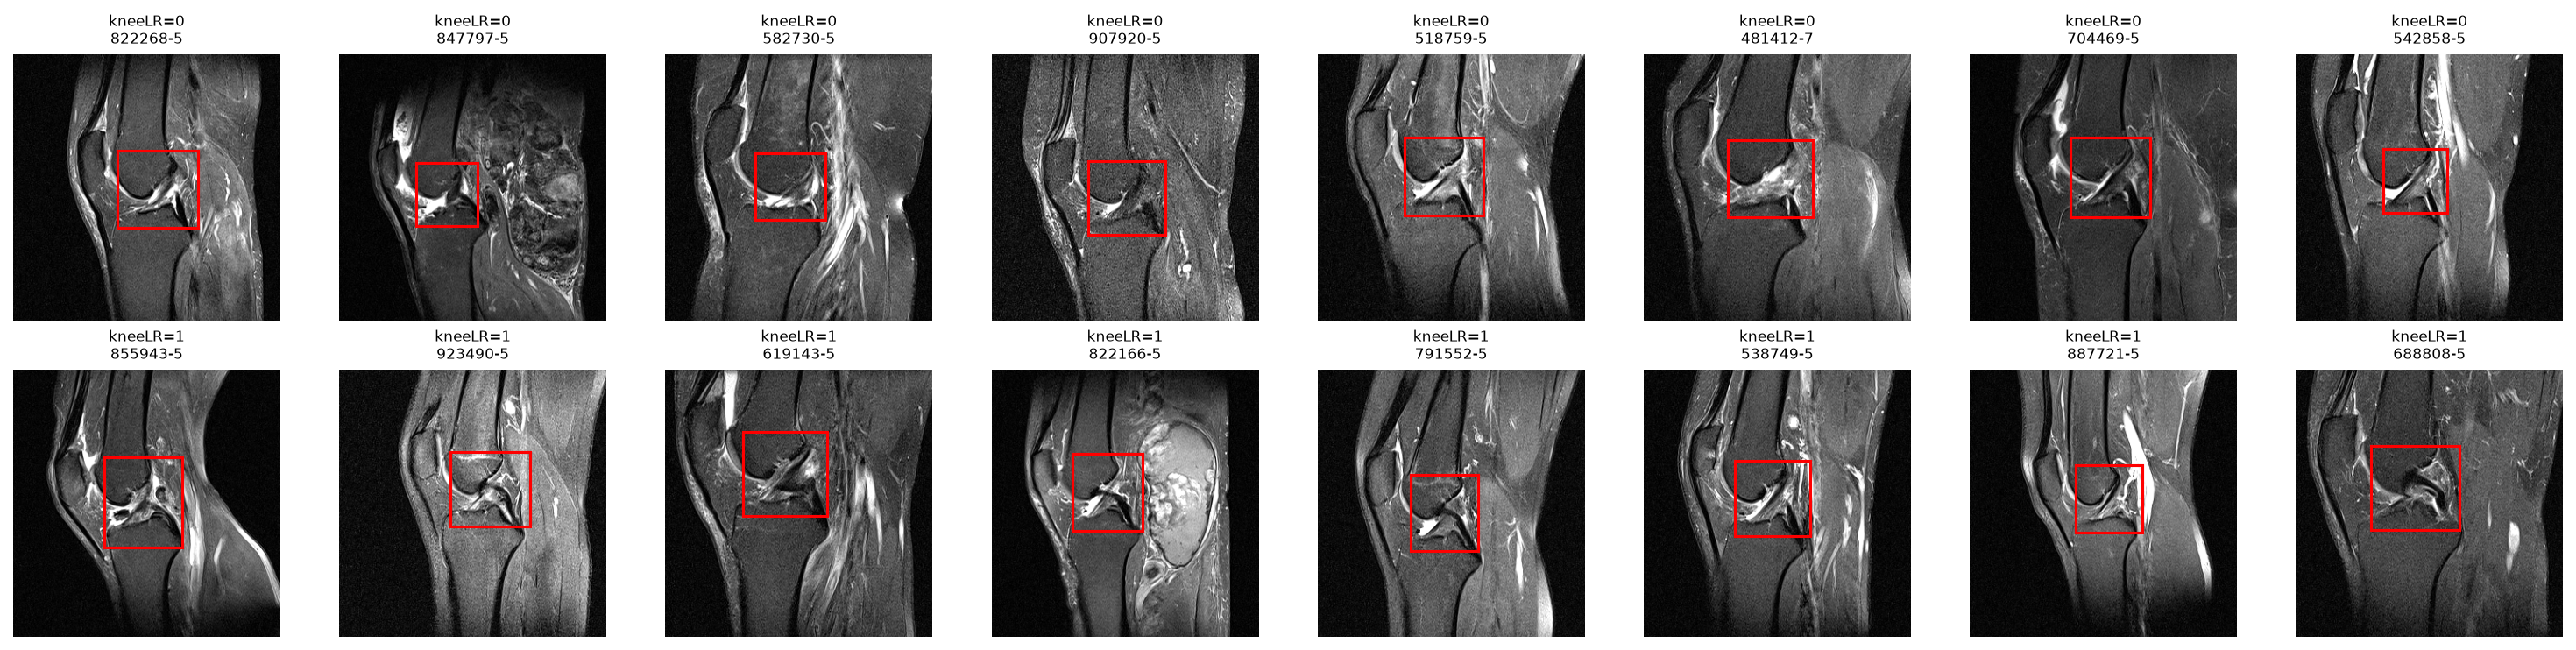
\includegraphics[width=\textwidth]{kneeLR.png}\\
  {\scriptsize\color{gris} Cortes centrales con la caja anotada del LCA (rojo).}
\end{frame}

% -------------------------------------------------------------------------
\begin{frame}{Cómo se planteó la solución}
  \centering
  \begin{tikzpicture}[
    node distance=0.4cm,
    paso/.style={draw=acento, rounded corners=3pt, fill=acento!8, align=center,
                 font=\small, minimum height=1.2cm, text width=2.0cm},
    arr/.style={-{Stealth[length=2mm]}, acento}
  ]
    \node[paso] (vol) {Volumen\\de RM};
    \node[paso, right=of vol] (cor) {Cada corte\\+ sus 2 vecinos};
    \node[paso, right=of cor] (red) {Red neuronal\\(ResNet-18)};
    \node[paso, right=of red] (sal) {¿Tiene LCA?\\+ caja 2D};
    \node[paso, right=of sal] (agg) {Se unen los\\cortes: caja 3D};
    \draw[arr] (vol) -- (cor);
    \draw[arr] (cor) -- (red);
    \draw[arr] (red) -- (sal);
    \draw[arr] (sal) -- (agg);
  \end{tikzpicture}

  \vspace{1.2em}
  \begin{columns}[T]
    \begin{column}{0.48\textwidth}
      \textbf{Métrica:} IoU, el solapamiento entre la caja predicha y la real
      (0 = no se tocan, 1 = idénticas).
    \end{column}
    \begin{column}{0.48\textwidth}
      \textbf{Resultado en prueba}\\ {\small(153 volúmenes nunca vistos)}\\[0.3em]
      \small
      \begin{tabular}{@{}lc@{}}
        Caja promedio fija (línea base) & 0.39 \\
        \textbf{Modelo} & \textbf{0.70} \\
        Meta del proyecto & $\geq 0.50$ \\
      \end{tabular}
    \end{column}
  \end{columns}
\end{frame}

% -------------------------------------------------------------------------
\begin{frame}{La pregunta de hoy: ¿el modelo mira donde debe?}
  \begin{itemize}
    \item Un buen IoU no garantiza que el modelo use el ligamento: podría apoyarse en
          atajos (posición típica de la rodilla, bordes, artefactos).
    \item \textbf{Grad-CAM} genera un mapa de calor con las zonas de la imagen
          que más influyeron en la decisión ``este corte tiene LCA''.
    \item Se midió sobre los 3063 cortes con LCA de validación cruzada:
      \begin{itemize}
        \item \textbf{Energía en la caja:} qué fracción del mapa cae dentro de la caja real.
              Por azar sería igual al área de la caja (${\approx}$\,8\,\% de la imagen).
        \item \textbf{Acierto del punto máximo:} si el punto más caliente del mapa cae dentro de la caja.
      \end{itemize}
    \item \textbf{Control:} la misma red \emph{sin entrenar}. Si también ``acierta'',
          el efecto no es aprendido.
  \end{itemize}
\end{frame}

% -------------------------------------------------------------------------
\begin{frame}{Casos con mejor IoU}
  \begin{columns}[c]
    \begin{column}{0.42\textwidth}
      \centering
      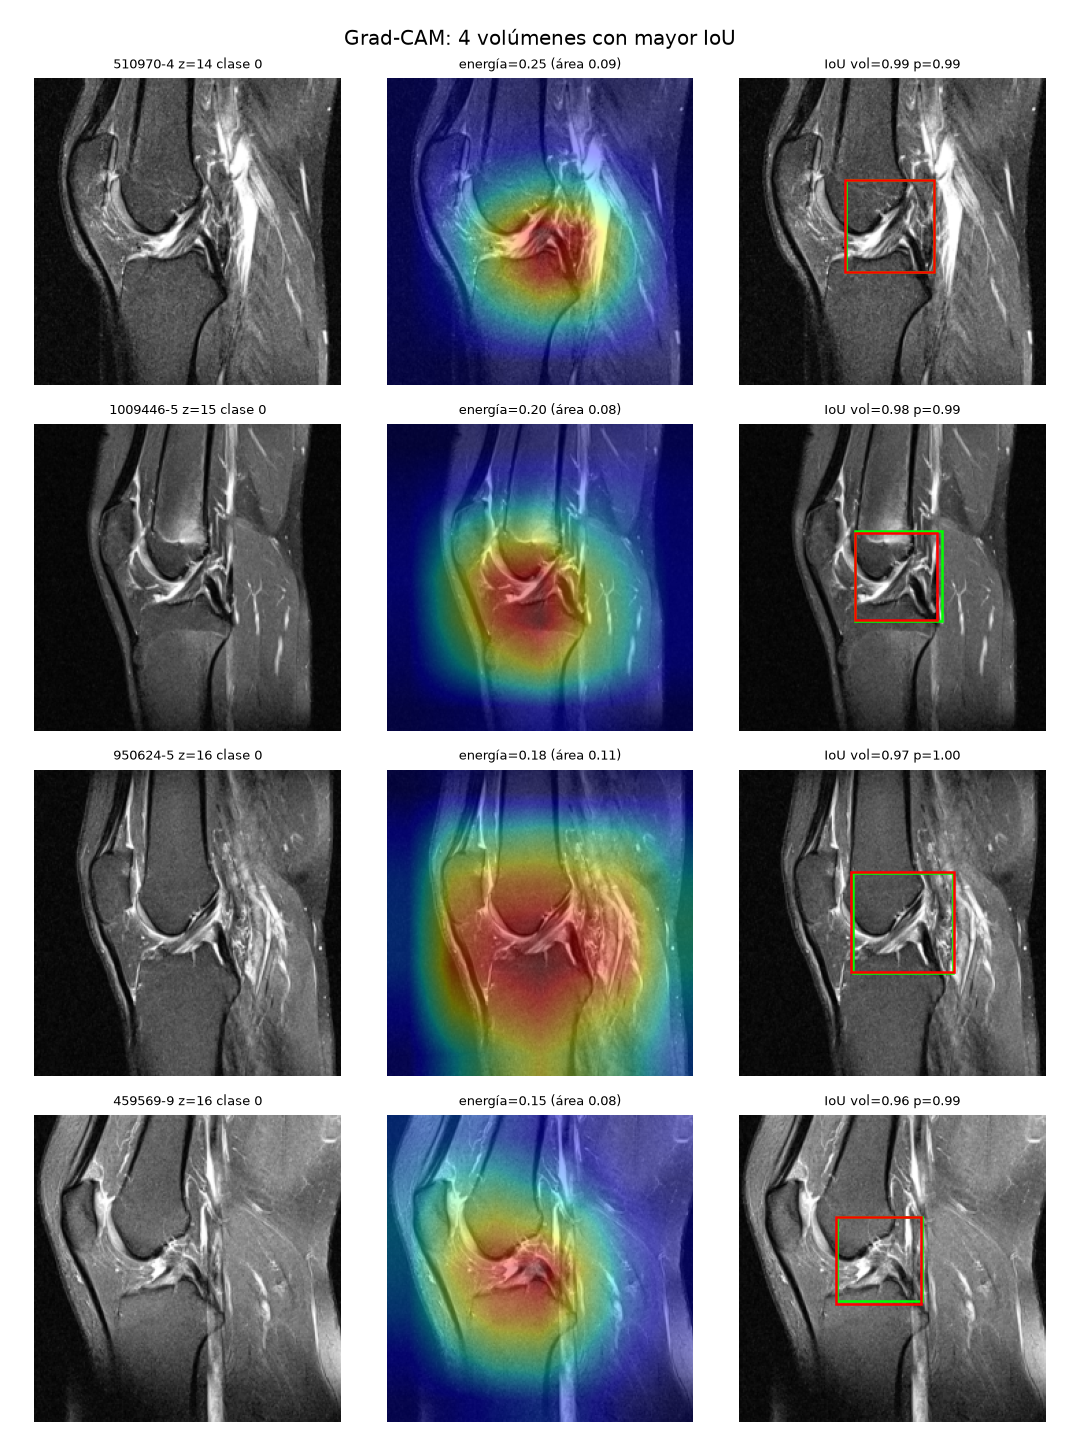
\includegraphics[height=0.86\textheight]{gradcam_best.png}
    \end{column}
    \begin{column}{0.55\textwidth}
      \small
      \begin{itemize}
        \item Columnas: corte original, mapa Grad-CAM, cajas.
        \item \textcolor{green!50!black}{\textbf{Verde}}: caja real.
              \textcolor{red}{\textbf{Rojo}}: caja predicha.
        \item El calor se concentra sobre la escotadura intercondílea,
              donde está el LCA.
        \item Energía en la caja: 15--25\,\% frente a 8--11\,\% por azar.
        \item El mapa es difuso: la red lo calcula en una rejilla de $7\times7$,
              así que no se ``dibuja'' el ligamento, se señala la región.
      \end{itemize}
    \end{column}
  \end{columns}
\end{frame}

% -------------------------------------------------------------------------
\begin{frame}{Casos con peor IoU}
  \begin{columns}[c]
    \begin{column}{0.42\textwidth}
      \centering
      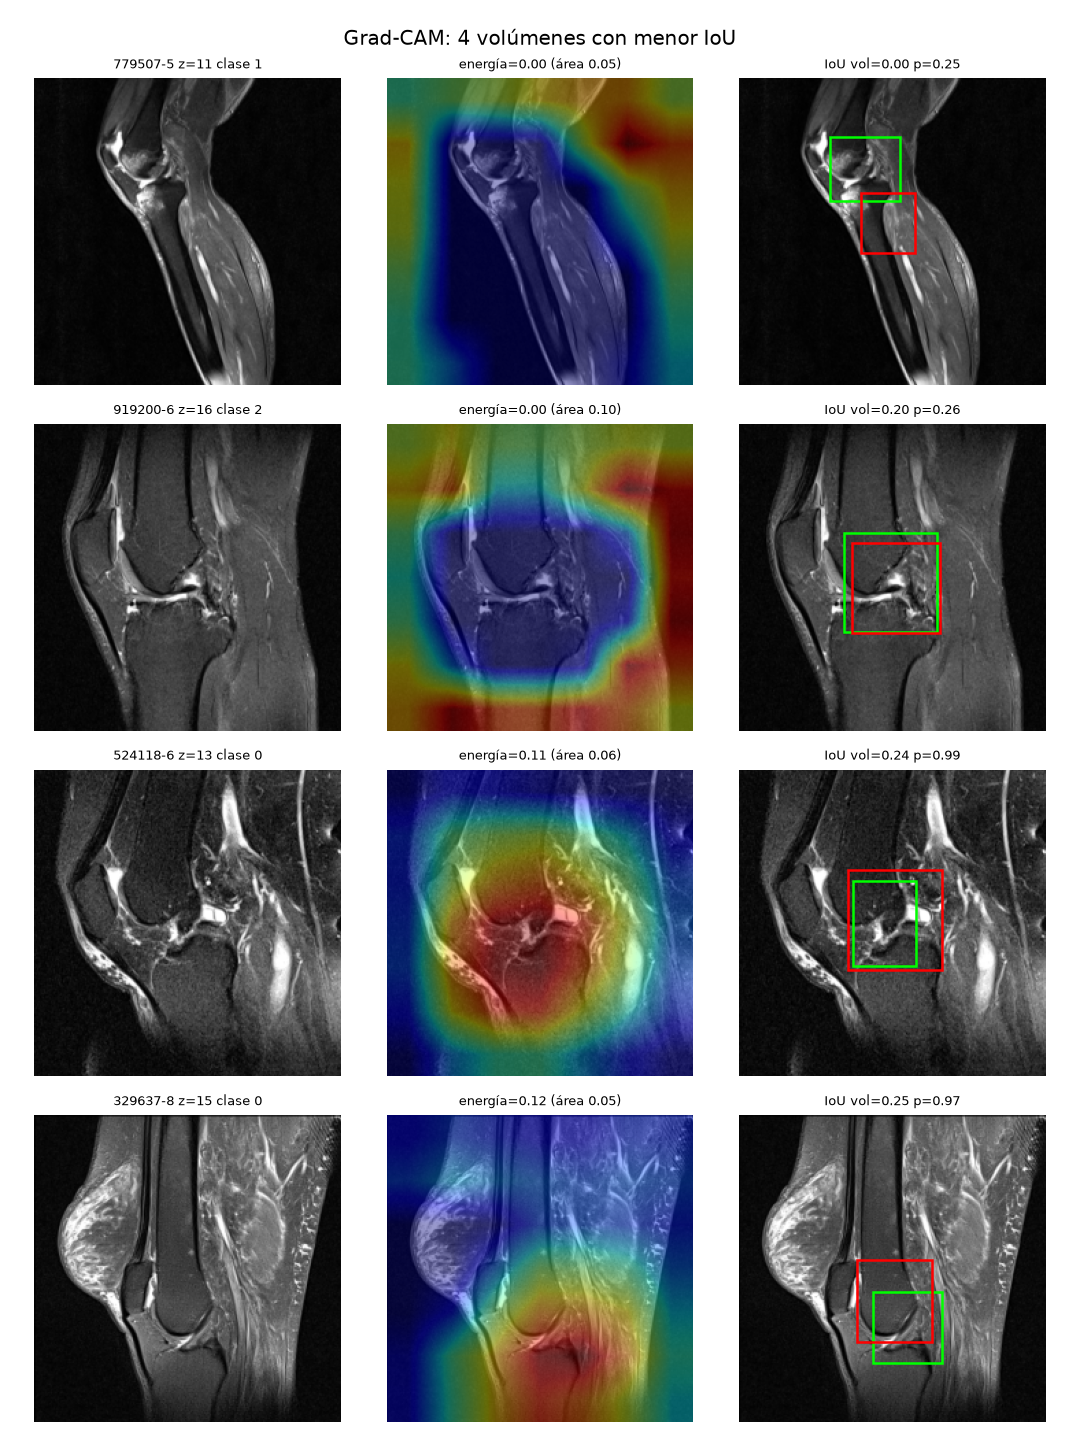
\includegraphics[height=0.86\textheight]{gradcam_worst.png}
    \end{column}
    \begin{column}{0.55\textwidth}
      \small
      \begin{itemize}
        \item Dos tipos de error:
          \begin{enumerate}
            \item \textbf{Baja confianza} ($p\approx0.25$): el modelo no reconoce el LCA
                  y el mapa se va a los bordes de la imagen.
            \item \textbf{Confianza alta, caja desplazada:} el mapa sí apunta a la rodilla,
                  pero la caja predicha queda corrida respecto a la real.
          \end{enumerate}
        \item Cuando la atención se dispersa, la caja también falla:
              el mapa ayuda a explicar los errores.
      \end{itemize}
    \end{column}
  \end{columns}
\end{frame}

% -------------------------------------------------------------------------
\begin{frame}{Resultados cuantitativos}
  \centering
  \barras{Energía dentro de la caja}{0.16}{0.081}{0.104}{0.117}\hspace{1.2cm}%
  \barras{Acierto del punto máximo}{0.85}{0.081}{0.207}{0.712}

  {\scriptsize\color{gris} Mismos 153 volúmenes (pliegue 0). Azar = área media de la caja.
   En los 5 pliegues el modelo entrenado alcanza 0.149 de energía y 0.71 de acierto.}

  \vspace{0.4em}
  \small
  \begin{itemize}
    \item En energía, el modelo entrenado supera al azar y a la red sin entrenar
          (intervalos bootstrap al 95\,\% por encima de cero).
    \item Donde más se separa es el \textbf{punto máximo}: 71\,\% frente a 21\,\%.
  \end{itemize}
\end{frame}

% -------------------------------------------------------------------------
\begin{frame}{Qué aprendimos}
  \begin{itemize}
    \item \textbf{Sí, el modelo mira el ligamento.} La atención cae en la caja real casi el doble
          de lo esperado por azar (1.8$\times$), y el punto máximo acierta en 7 de cada 10 volúmenes.
    \item \textbf{La atención se relaciona con la calidad de la caja:} cuanto más concentrado está el mapa
          en el LCA, mejor el IoU (correlación 0.18, positiva). En la red sin entrenar no aparece.
    \item \textbf{Matices honestos:}
      \begin{itemize}
        \item Una red sin entrenar ya supera un poco al azar: parte del efecto viene de que la rodilla
              ocupa el centro de la imagen, no del aprendizaje.
        \item Se esperaba 3--5$\times$ el azar; se obtuvo 1.8$\times$, en parte por la baja resolución del mapa.
        \item Hay variación entre pliegues (energía de 0.12 a 0.21).
      \end{itemize}
  \end{itemize}
  \vspace{0.5em}
  \textbf{Próximos pasos:} script de predicción para casos nuevos, regla de monitoreo,
  artículo y presentación final (27 de noviembre).
\end{frame}

\end{document}
